\documentclass{article}
\usepackage{graphicx} % Required for inserting images
\graphicspath{https://www.overleaf.com/project/648ab1deeb9fb7e98482122e/file/648ab2e722026a5b7e69752f}
\graphicspath{https://www.overleaf.com/project/648ab1deeb9fb7e98482122e/file/648ab7e87516cd90d55fb69e}
\graphicspath{https://www.overleaf.com/project/648ab1deeb9fb7e98482122e/file/648abb2695097560ac072a08}
\graphicspath{https://www.overleaf.com/project/648ab1deeb9fb7e98482122e/file/648abc27817d0ae1e9139088}
\usepackage[a4paper, total={6in, 8in}]{geometry}


\begin{document}
\begin{center}
\begin{figure}
\centering

\includegraphics[scale = 0.35]{image.png}\\
The AI-ML and Data Science Club of IITH
\end{figure}
\end{center}

\begin{center}
   {\LARGE{\textbf{Introduction to Multi-Arm Bandits}}} 
\end{center}


\graphicspath{{./media/}}
\begin{center}
    \large{\textbf{{Contents}}}
\end{center}



\begin{enumerate}
 \item {What is Reinforcement Learning?}\\
 \item {What are Multi-Arm Bandits?}\\
 \item {What is Multi-Arm Bandit Problem?}\\
 \item {Types of Multi-Arm Bandits}\\
 \item {Exploration vs Exploitation trade-off in multi-arm bandits
}\\
 \item {Conclusion}\\
\end{enumerate}

\begin{center}
    \textbf{Compiled by :}
    \texttt{Sriram Gonella}
\end{center}


\newpage
\section{What is Reinforcement Learning?}
Reinforcement learning is a subfield of artificial intelligence that involves learning how to take actions in an environment in order to maximize a cumulative reward signal. It has become increasingly popular in recent years, with applications ranging from robotics to game playing to recommendation systems. At the heart of reinforcement learning is the notion of trial-and-error learning, where an agent interacts with its environment, learns from experience, and adjusts its behavior accordingly. Reinforcement learning is a machine learning type involving an agent learning to take actions in an environment to maximize a reward signal. To understand it better, let's consider the following example:
Imagine you are training a dog to do the trick. Every time the dog performs the trick correctly, you give it a treat. The dog aims to achieve the trick as often as possible to get as many treats as possible. The dog learns to associate performing the trick with receiving pleasure, so it starts to perform the trick more frequently.
In this example, the dog is the agent, the trick is the action, the treat is the reward, and the environment is the training area. Reinforcement learning works similarly. The agent interacts with the environment by taking steps, and the environment responds by providing a reward signal. The agent aims to learn the optimal policy, a set of actions that maximizes the expected reward.

\begin{center}
    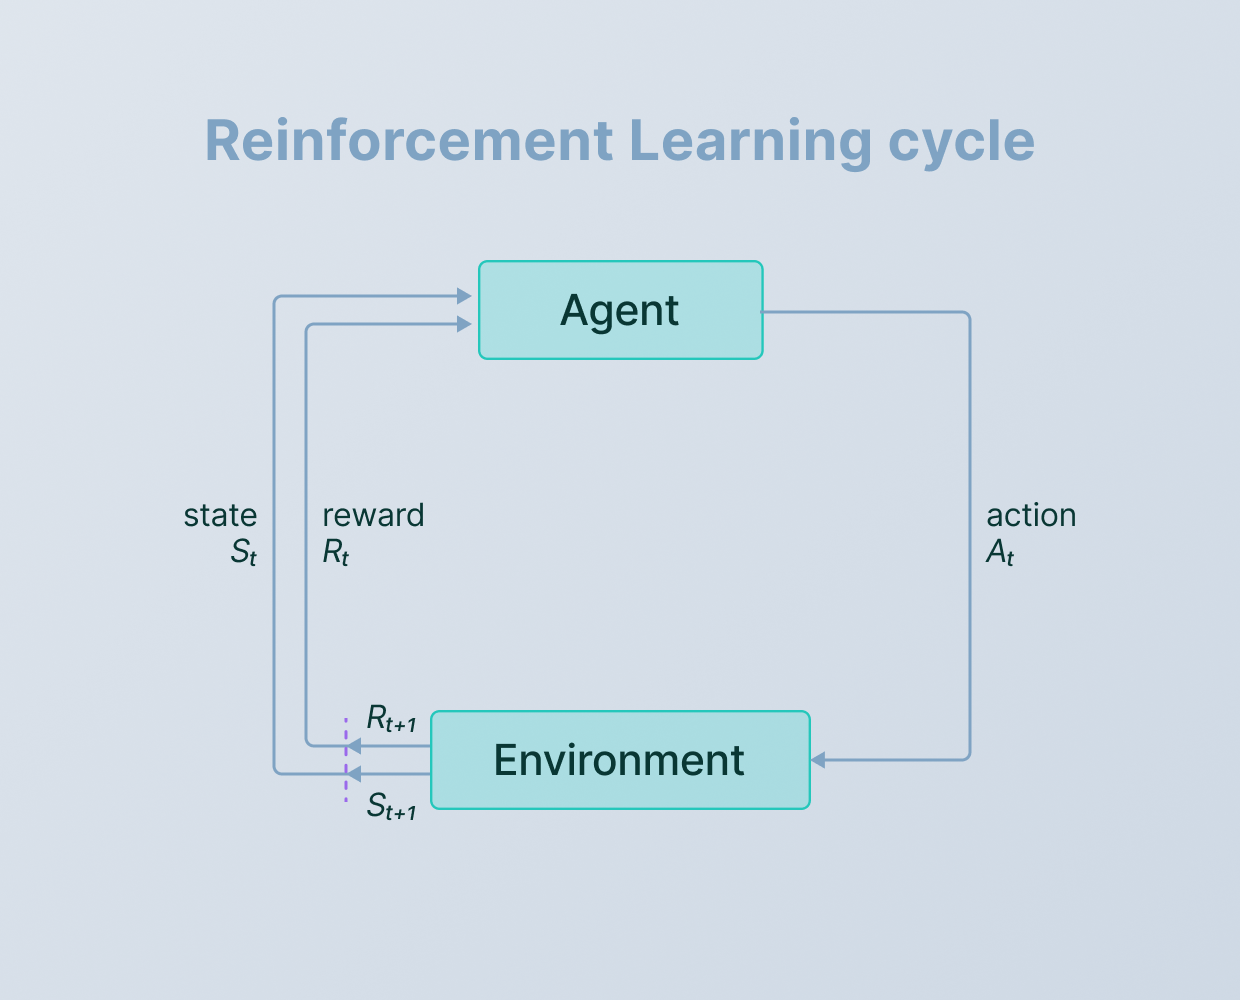
\includegraphics[scale = 0.55]{rlcycle.png}
\end{center}

\section{What are Multi-Arm Bandits?}
The term "bandit" comes from the idea of a slot machine or one-armed bandit in a casino, a machine that takes in money and returns a small portion of it as a reward, but the exact amount of the reward is uncertain and unknown.
In the context of machine learning, a "multi-armed bandit" refers to a problem where an agent has to make a decision from a set of options (or "arms") with uncertain rewards, just like a gambler pulling the arm of a slot machine.
The term "bandit" is used in this context because the agent is faced with a similar dilemma as a gambler: they have to choose between different options with uncertain rewards, and they have to balance the exploration of new opportunities to learn which one provides the highest reward with the exploitation of the current best option to maximize overall reward.

\begin{center}
    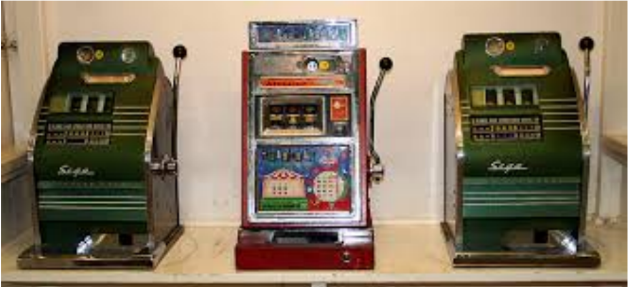
\includegraphics{slotmachine.png}
\end{center}

One classic example of reinforcement learning is the multi-armed bandit problem, which involves a decision-maker, or agent, who must choose between several different options, or "arms", each of which has an unknown probability of yielding a reward. The goal is to learn which arm is the most rewarding through a process of exploration and exploitation, balancing the need to explore new options with the desire to maximize reward.

For example, consider a scenario where a news website wants to maximize the number of clicks on its articles. The website could use a multi-armed bandit algorithm to determine which articles to display on its front page, with each article being an "arm" that the algorithm can choose to "pull" or display to a user. By tracking which articles receive the most clicks over time, the algorithm can learn which articles are the most popular and adjust its selection accordingly to maximize clicks.

In this way, the multi-armed bandit problem serves as a simple but powerful model for many real-world decision-making scenarios, and has become a fundamental concept in the study of reinforcement learning.

\section{What is Multi-Arm Bandit Problem?}
The multi-armed bandit problem is a classic reinforcement learning problem where an agent has to decide between multiple actions, each with an unknown reward distribution, to maximize its total reward over time. The name "bandit" comes from the idea of a gambler facing multiple slot machines (or "one-armed bandits") with unknown payout rates and trying to decide which one to play to maximize their total winnings.
More formally, in a multi-armed bandit problem, there are N actions or "arms" and each arm has an unknown reward distribution. At each time step, the agent chooses an arm to play and observes the reward associated with that arm. The goal is to maximize the total reward over a fixed number of time steps while learning the reward distributions of the arms.
Here is an example of a multi-armed bandit problem:
Suppose you are an online advertising company, and you have several ad designs that you can show to users. Each ad has an unknown click-through rate (CTR), which represents the probability that a user will click on the ad. You want to maximize the total number of clicks over a fixed number of impressions (i.e., times the ad is shown) while learning the CTRs of the different ad designs. Each time a user visits your website, you can choose which ad to show them and observe whether or not they click on the ad.
Another example could be a healthcare setting where doctors have multiple treatment options to treat a specific condition, and each treatment has an unknown probability of success. The goal is to choose the treatment that maximizes the overall success rate while also learning the success rate of each treatment.
The multi-armed bandit problem arises in many real-world applications with multiple choices and limited resources. Finding the best choice while learning about each option's reward distribution is a common challenge in many fields, including marketing, finance, and healthcare.

\begin{center}
    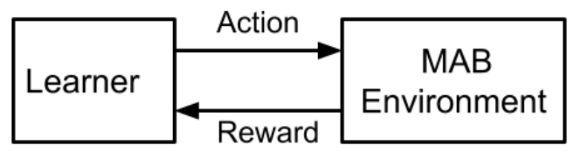
\includegraphics{MABcycle.png}
\end{center}

\section{Types of Multi-Arm Bandits}
There are different types of multi-armed bandit problems that can arise in different contexts. Here are the most common types:

\begin{enumerate}
    
\item $\textbf{Stochastic Multi-Armed Bandits:}$ In this type of bandit problem, the reward distribution of each arm is fixed but unknown to the agent. The rewards are generated randomly from a fixed distribution each time an arm is played. The goal is to learn the expected reward distribution of each arm and then choose the arm with the highest expected reward. 

\item $\textbf{Adversarial Multi-Armed Bandits:}$ In this type of bandit problem, the rewards of each arm are chosen by an adversary who tries to make it as difficult as possible for the agent to maximize its total reward. The reward distribution of each arm can change over time based on the agent's choices. The goal is to develop a strategy that minimizes the regret, which is the difference between the total reward obtained by the agent and the total reward that would have been obtained if the agent had chosen the best arm every time.

\item $\textbf{Contextual Multi-Armed Bandits:}$ In this type of bandit problem, each arm is associated with a set of contextual features, and the reward of each arm depends on these features. The goal is to learn a model that maps the contextual features to the expected reward for each arm and then choose the arm with the highest expected reward based on the current context. 

\item $\textbf{Semi-Bandits:}$ In this type of bandit problem, the agent can observe some partial information about the rewards of the other arms before making its choice. This partial information can be used to make a more informed decision. The goal is to develop a strategy that maximizes the total reward given the partial information.
\end{enumerate}

These different types of multi-armed bandit problems require different strategies and algorithms to solve. Depending on the context and available information, one may need to use a combination of these approaches to find the best solution.

\section{Exploration vs Exploitation trade-off in multi-arm bandits}
Exploration vs. Exploitation is a fundamental trade-off in multi-arm bandit problems. The problem is to choose among multiple options, each with uncertain rewards. The exploration vs. exploitation trade-off involves deciding whether to try out new options to gain information about their rewards or to choose the option with the highest available reward to maximize overall rewards.

\begin{center}
    
\includegraphics[scale = 0.75]{exploration-exploitation-balance-pictured-balanced-260nw-1586195143 (1).jpg}
\end{center}

$\textbf{Exploration:}$ Exploring new options to gain information about their rewards is called exploration. Exploration involves taking risks and trying out new options with uncertain rewards. Exploration aims to gain information about the rewards of different options, which can lead to better decisions in the long run. However, exploration may lead to immediate lower rewards.

$\textbf{Exploitation:}$ Exploitation involves selecting the option with the highest available reward to maximize immediate rewards. Exploitation consists in making a decision based on the current information without exploring other options. Exploitation may lead to suboptimal decisions in the long run if there are better options than the highest available reward.

Here is an example to illustrate the exploration vs. exploitation trade-off in multi-arm bandit problems:
Imagine you are a marketer and must choose which ad to display to users. Each ad has an unknown click-through rate (CTR), the reward. The goal is to maximize overall rewards by selecting the advertisement with the highest CTR.
At the beginning of the campaign, you need to have information about the CTR of each ad, so you have to explore. You might start by randomly selecting ads to display to users and collecting data on their CTRs. This exploration phase will help you gain information about the CTRs of different ads.
Once you have some information about the CTRs of each ad, you can start exploiting the option with the highest known CTR. You can continue to exploit this option until you gain more information about the CTRs of other ads, which might lead you to explore again.
The key challenge in multi-arm bandit problems is to balance exploration and exploitation to maximize overall rewards. Choosing too much exploration may lead to low immediate rewards, while choosing too much exploitation may lead to suboptimal decisions in the long run.

\section{Conclusion}
In conclusion, multi-armed bandits are a powerful framework for solving decision-making problems in many real-world scenarios. We started with an introduction to the concept of multi-armed bandits and their importance in the field of reinforcement learning. We then explored the different types of multi-armed bandits, such as stochastic, adversarial, contextual, and semi-bandits, and discussed how they differ in terms of the information available to the agent and the nature of the rewards. We also discussed the exploration-exploitation tradeoff, which is a fundamental concept in multi-armed bandits, where the agent must balance the need to explore new options with the desire to maximize reward. This tradeoff is at the heart of many multi-armed bandit algorithms.

In the next article, we will dive deeper into the algorithms used to solve multi-armed bandit problems. We will discuss some of the most popular algorithms used in practice, such as Epsilon-Greedy, Upper Confidence Bound (UCB), and Thompson Sampling. We will explain how these algorithms work, their strengths and weaknesses, and provide examples of how they can be used in real-world scenarios.

Overall, the study of multi-armed bandits is an exciting area of research with many practical applications, and we hope that this article has provided a useful introduction to the topic. 

\end{document}
